\chapter{Introduzione}

L'annegamento rappresenta ancora oggi un problema di rilevanza mondiale, nonostante i progressi compiuti nell'ambito della prevenzione, della sorveglianza e delle tecniche di soccorso. Secondo l'ultimo \emph{report} pubblicato dall'Organizzazione Mondiale della Sanità (OMS), datato al 1° maggio 2026, ogni anno si registrano a livello globale circa 300\,000 decessi riconducibili all'annegamento \cite{WHO2026Drowning}. Il fenomeno assume una rilevanza ancora maggiore se si considera la distribuzione delle vittime per fascia d'età: l'annegamento si colloca infatti tra le principali cause di morte nell'infanzia, risultando la quarta causa di morte per i bambini di età compresa tra 1 e 4 anni e la terza per quelli appartenenti alla fascia tra 5 e 14 anni \cite{WHO2026Drowning}.

Questi dati evidenziano come l'annegamento non costituisca un fenomeno marginale, ma un problema di sicurezza che interessa in modo particolarmente significativo le fasce più giovani della popolazione. La prevenzione assume pertanto un ruolo centrale e comprende sia interventi di carattere organizzativo e infrastrutturale, sia l'adozione di strumenti tecnologici capaci di supportare il personale addetto alla sorveglianza \cite{WHO2026Drowning,UNI20380}.

Accanto agli interventi di prevenzione, assume quindi particolare rilievo la tempestività con cui una situazione di pericolo viene riconosciuta e vengono avviate le operazioni di soccorso. Da questa esigenza deriva un interesse collettivo per lo sviluppo di sistemi automatici capaci di affiancare la normale attività di vigilanza, analizzando continuativamente quanto avviene all'interno della vasca e segnalando situazioni potenzialmente compatibili con un episodio di crisi \cite{Eng2008DEWS,UNI20380}.

Il presente elaborato si colloca dunque in questo ambito e affronta, in particolare, il problema della rilevazione automatica dei bagnanti, all'interno di un più ampio sistema destinato alla rilevazione precoce di potenziali fenomeni di annegamento.

\section{Il problema dell'annegamento}

Pur offrendo un inquadramento generale del fenomeno, i dati globali non esauriscono gli aspetti rilevanti ai fini di questo lavoro, che si concentra sugli incidenti avvenuti nelle piscine. Rispetto alle acque libere, le piscine costituiscono ambienti più controllati e, proprio per questo, particolarmente adatti all'impiego di sistemi di videosorveglianza automatizzata \cite{UNI20380}.

Nel contesto italiano, il rapporto sugli annegamenti pubblicato da Federalberghi nel giugno 2026, stima che tra il 1° gennaio 2022 e il 31 maggio 2026 si siano verificati complessivamente 63 annegamenti in piscina, corrispondenti a una media di circa 14 casi all'anno. Il dato comprende differenti tipologie di struttura, tra cui piscine di centri sportivi, parchi acquatici, piscine comunali, stabilimenti termali, strutture ricettive e abitazioni private \cite{Federalberghi2026}.

La stessa analisi evidenzia una particolare incidenza del fenomeno sulle fasce di età più giovani. Dei 63 casi considerati, il 57,2\% degli episodi censiti riguarda soggetti con un'età inferiore a quindici anni \cite{Federalberghi2026}. Tali dati forniscono un'indicazione significativa della persistenza del problema anche all'interno di ambienti strutturati e sottoposti a forme di sorveglianza.

\begin{table}[htbp]
    \centering
    \caption{Annegamenti avvenuti nelle piscine italiane da gennaio 2022 a maggio 2026, per fascia d'età e sesso}
    \label{tab:annegamenti-eta-sesso}
    \small
    \renewcommand{\arraystretch}{1.15}
    \begin{tabularx}{\textwidth}{|>{\raggedright\arraybackslash}X||>{\centering\arraybackslash}m{1.5cm}|>{\centering\arraybackslash}m{1.5cm}|>{\centering\arraybackslash}m{1.5cm}|>{\centering\arraybackslash}m{1.5cm}|>{\centering\arraybackslash}m{1.5cm}|>{\centering\arraybackslash}m{1.5cm}|}
        \hline
        Fascia d'età & Maschi & \% & Femmine & \% & Totale & \% \\
        \hline\hline
        Sino a 4 anni  & 15 & 31,9\% & 2 & 12,5\% & 17 & 27,0\% \\
        \hline
        5--14 anni    & 12 & 25,5\% & 7 & 43,8\% & 19 & 30,2\% \\
        \hline
        15--24 anni   & 7  & 14,9\% & 1 & 6,3\%  & 8  & 12,7\% \\
        \hline
        25--44 anni   & 6  & 12,8\% & 0 & 0,0\%  & 6  & 9,5\% \\
        \hline
        45--64 anni   & 2  & 4,3\%  & 2 & 12,5\% & 4  & 6,3\% \\
        \hline
        65 anni e oltre & 5 & 10,6\% & 4 & 25,0\% & 9 & 14,3\% \\
        \hline
        Totale        & 47 & 100,0\% & 16 & 100,0\% & 63 & 100,0\% \\
        \hline
        \%            & 74,6\% & & 25,4\% & & 100,0\% & \\
        \hline
    \end{tabularx}

\end{table}

\begin{table}[htbp]
    \centering
    \caption{Annegamenti avvenuti nelle piscine italiane da gennaio 2022 a maggio 2026, per fascia d'età e tipologia di piscina}
    \label{tab:annegamenti-eta-tipologia-piscina}
    \small
    \renewcommand{\arraystretch}{1.15}
    \begin{tabularx}{\textwidth}{|>{\raggedright\arraybackslash}X||>{\centering\arraybackslash}m{2.3cm}|>{\centering\arraybackslash}m{2.3cm}|>{\centering\arraybackslash}m{2.3cm}|>{\centering\arraybackslash}m{1.4cm}|>{\centering\arraybackslash}m{1.4cm}|}
        \hline
        Fascia d'età & Aperte al pubblico & Annesse ad abitazioni & Riservate agli alloggiati & Totale & \% \\
        \hline\hline
        Sino a 4 anni  & 4  & 11 & 2 & 17 & 27,0\% \\
        \hline
        5--14 anni     & 13 & 0  & 6 & 19 & 30,2\% \\
        \hline
        15--24 anni    & 2  & 3  & 3 & 8  & 12,7\% \\
        \hline
        25--44 anni    & 2  & 3  & 1 & 6  & 9,5\% \\
        \hline
        45--64 anni    & 3  & 1  & 0 & 4  & 6,3\% \\
        \hline
        65 anni e oltre & 4 & 0  & 5 & 9  & 14,3\% \\
        \hline
        Totale         & 28 & 18 & 17 & 63 & 100,0\% \\
        \hline
        \%             & 44,4\% & 28,6\% & 27,0\% & 100,0\% & \\
        \hline
    \end{tabularx}

\end{table}

La presenza di personale addetto alla vigilanza rappresenta naturalmente la principale forma di prevenzione all'interno delle piscine pubbliche.\footnote{La norma UNI EN ISO 20380:2018 stabilisce che i sistemi di visione computerizzata sono progettati per integrare il bagnino o il personale addestrato e non per ridurre la sorveglianza umana \cite{UNI20380}.} L'utilizzo di un sistema automatico di rilevazione non deve quindi essere interpretato come una sostituzione del bagnino, bensì come un ulteriore livello di sicurezza in grado di affiancarne l'attività.

L'utilità di un simile strumento deriva anche dalle peculiarità con cui può manifestarsi un episodio di annegamento. La rappresentazione comunemente associata a questo fenomeno, caratterizzata necessariamente da movimenti estremamente vistosi e da esplicite richieste di aiuto, non descrive infatti tutte le situazioni possibili \cite{Pia1974Observation,Pia1999Reflections,PascualGomez2022Recognition}. Ai fini della progettazione di un sistema di visione artificiale è quindi necessario identificare quali caratteristiche del comportamento del bagnante possano essere effettivamente osservate attraverso una sequenza video.

\subsection{Manifestazioni osservabili dell'annegamento}

L'analisi viene condotta principalmente in senso visivo-comportamentale: l'obiettivo non è formulare una descrizione clinica del processo di annegamento, bensì individuare i segnali esteriori osservabili da un operatore o acquisibili mediante una telecamera, rilevanti per un sistema automatico di rilevazione.

Le assunzioni comportamentali utilizzate all'interno del progetto derivano principalmente dagli studi di Frank Pia sul comportamento dei soggetti in difficoltà in acqua \cite{Pia1974Observation,Pia1999Reflections}, successivamente ripresi nell'architettura di riferimento adottata nel presente lavoro \cite{Kam2002Drowning,Eng2008DEWS}. Questi studi hanno avuto un ruolo centrale nella definizione di indicatori visivi utilizzabili per distinguere una normale attività natatoria da una situazione di crisi. Studi osservazionali e revisioni più recenti hanno tuttavia evidenziato una maggiore varietà delle manifestazioni visibili e una disponibilità ancora limitata di evidenze empiriche sui segnali precoci \cite{CarballoFazanes2020VisibleBehaviour,PascualGomez2022Recognition}. Gli indicatori descritti di seguito devono quindi essere intesi come il modello di riferimento adottato dal sistema in analisi, non come criteri sufficienti a riconoscere ogni possibile episodio.

Una prima distinzione rilevante riguarda i concetti di \emph{distress} e di \emph{drowning}. Nel primo caso il soggetto si trova in una situazione di difficoltà e non è in grado di raggiungere autonomamente una condizione di sicurezza, ad esempio a causa di stanchezza o di altre condizioni contingenti, ma conserva almeno parzialmente il controllo volontario dei propri movimenti \cite{Pia1999Reflections,Kam2002Drowning}.

La situazione di annegamento propriamente detta presenta invece caratteristiche differenti. In particolare, gli indicatori descritti di seguito si riferiscono alla forma attiva dell'annegamento, nella quale il soggetto manifesta una risposta comportamentale istintiva, indicata come \emph{instinctive drowning response}, associata alla condizione di soffocamento in acqua \cite{Pia1974Observation,Pia1999Reflections,Eng2008DEWS}. In questa fase il comportamento del soggetto non corrisponde necessariamente a una serie di azioni volontarie finalizzate alla richiesta di soccorso, ma è dominato dal tentativo di mantenere le vie respiratorie al di sopra della superficie.

Dal punto di vista osservabile, i principali indicatori considerati possono essere riassunti nei seguenti elementi \cite{Pia1974Observation,Pia1999Reflections,Kam2002Drowning,PascualGomez2022Recognition}:

\begin{itemize}
    \item il corpo tende ad assumere una posizione prevalentemente verticale rispetto alla superficie dell'acqua;
    
    \item lo spostamento orizzontale o diagonale del soggetto risulta limitato, dal momento che il movimento prodotto non è efficace nel generare una normale progressione natatoria;
    
    \item le braccia possono presentare movimenti ripetitivi, orientati lateralmente o frontalmente e caratterizzati dal tentativo di spingere verso il basso la superficie dell'acqua;
    
    \item l'azione degli arti inferiori può risultare assente, irregolare oppure inefficace ai fini della propulsione;
    
    \item la testa può risultare reclinata all'indietro, nel tentativo di mantenere bocca e naso al di sopra della superficie dell'acqua;

    \item il controllo volontario dei movimenti risulta fortemente limitato e il soggetto può non essere in grado di chiamare aiuto, poiché l'attività è principalmente finalizzata a mantenere la respirazione;
    
    \item il soggetto può alternare fasi di immersione ed emersione, fino all'eventuale completa sommersione;
    
    \item la fase di lotta in superficie costituisce un fenomeno temporalmente circoscritto: negli studi di Pia viene indicata una durata approssimativa compresa tra 20 e 60 secondi \cite{Pia1974Observation,Pia1999Reflections}.
\end{itemize}

\begin{figure}[htbp]
    \centering
    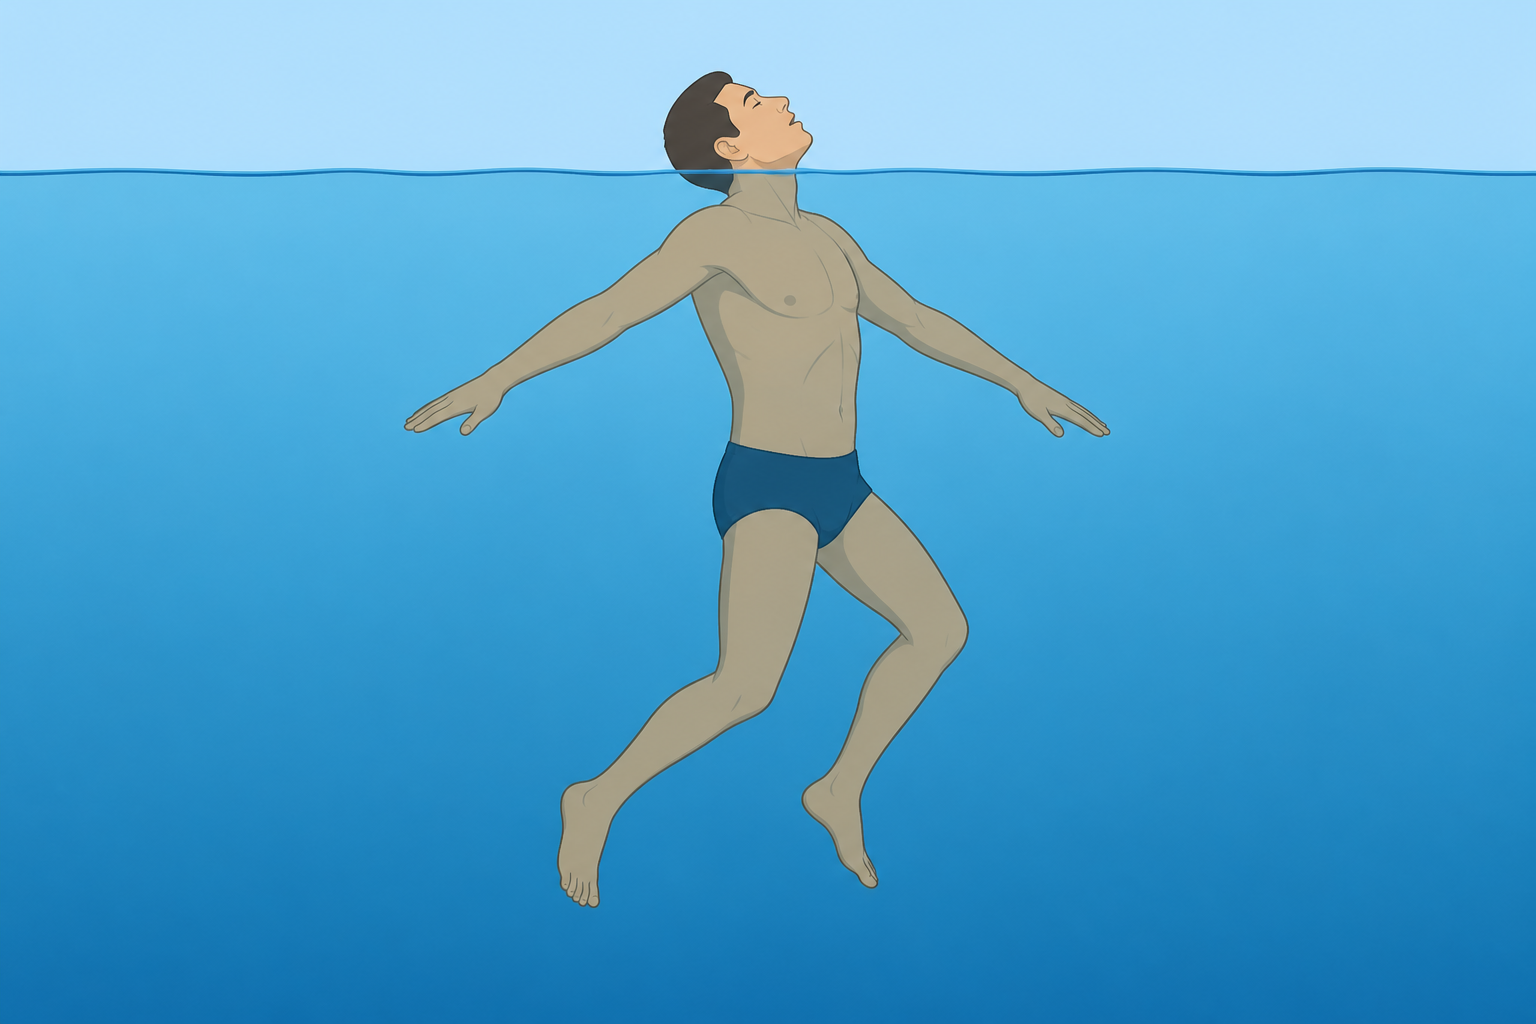
\includegraphics[width=0.72\textwidth]{figures/manifestazioni-annegamento-attivo.png}
    \caption{Rappresentazione delle principali manifestazioni osservabili dell'annegamento attivo}
    \label{fig:manifestazioni-annegamento-attivo}
\end{figure}

Proprio quest'ultimo elemento evidenzia l'importanza della rilevazione precoce. Un sistema che sia in grado di individuare soltanto la presenza di un corpo ormai immobile sul fondo della vasca interviene infatti in una fase successiva rispetto a un sistema capace di osservare e interpretare il comportamento del bagnante mentre la crisi è ancora in corso. Questo principio costituisce una delle motivazioni alla base della scelta, nell'architettura di riferimento, di utilizzare telecamere installate al di sopra della piscina anziché affidarsi esclusivamente a dispositivi subacquei \cite{Eng2003Automatic,Eng2006Robust,Eng2008DEWS}.

Accanto alla condizione di annegamento caratterizzata da una risposta attiva viene inoltre considerata una forma passiva. Con \emph{passive drowning} si indica una condizione nella quale il soggetto, a seguito di una perdita di coscienza, scivola sott'acqua senza manifestare movimenti di lotta o richieste di aiuto evidenti. Tale condizione può presentarsi direttamente oppure costituire l'evoluzione di una fase inizialmente attiva, quando i movimenti di lotta cessano e il soggetto non riesce più a mantenersi in superficie. Le due condizioni risultano quindi profondamente differenti dal punto di vista della loro apparenza visiva: la prima è caratterizzata soprattutto dall'analisi del movimento e della postura, mentre nella seconda assumono maggiore importanza la progressiva sommersione e l'assenza di un'attività natatoria efficace \cite{Kam2002Drowning,Lu2004Vision}.

\begin{table}[htbp]
    \centering
    \caption{Confronto tra le manifestazioni osservabili dell'annegamento attivo e passivo}
    \label{tab:confronto-annegamento-attivo-passivo}
    \small
    \renewcommand{\arraystretch}{1.15}
    \begin{tabularx}{\textwidth}{|>{\raggedright\arraybackslash}m{2.8cm}||>{\raggedright\arraybackslash}X|>{\raggedright\arraybackslash}X|}
        \hline
        Caratteristica & Annegamento attivo & Annegamento passivo \\
        \hline\hline
        Stato di coscienza & Generalmente cosciente durante la fase di lotta & Perdita di coscienza \\
        \hline
        Manifestazioni osservabili & Movimenti di lotta e tentativo di mantenere le vie respiratorie emerse & Assenza di lotta e progressiva sommersione \\
        \hline
        Postura e movimento & Posizione prevalentemente verticale, movimenti laterali delle braccia e propulsione inefficace & Assenza di movimenti volontari; corpo immobile o soggetto a spostamenti indotti dall'acqua \\
        \hline
        Evoluzione & Può terminare con la completa sommersione ed evolvere nella forma passiva & Può manifestarsi direttamente oppure seguire una precedente fase attiva \\
        \hline
        Principali indicatori & Postura, movimenti ripetitivi e alternanza tra immersione ed emersione & Progressiva sommersione, immobilità e assenza di movimenti volontari \\
        \hline
    \end{tabularx}

\end{table}

Tale variabilità costituisce uno dei principali problemi di un sistema automatico. Non esiste infatti un singolo attributo visivo sufficiente a identificare con certezza ogni possibile situazione di annegamento. Di conseguenza, la rilevazione di una crisi richiede l'osservazione congiunta di più caratteristiche e, soprattutto, della loro evoluzione nel tempo.

\section{Obiettivi dell'elaborato}

A partire dalle considerazioni precedenti, il presente elaborato affronta lo sviluppo di un sistema di visione artificiale per la rilevazione precoce di potenziali incidenti da annegamento in piscina. Il principale riferimento architetturale è il \textit{Drowning Early Warning System} (DEWS), un sistema basato su telecamere sopraelevate e progettato per riconoscere i bagnanti e analizzarne il comportamento in tempo reale al fine di identificare situazioni di \emph{water crisis} \cite{Eng2008DEWS}.

L'ambiente acquatico presenta difficoltà specifiche: riflessi, increspature, schizzi, ombre, movimenti delle corsie e variazioni dell'illuminazione modificano continuamente l'immagine anche in assenza di persone. Per gestire tale variabilità, il modulo di rilevazione originale impiega modelli statistici e diverse procedure deterministiche, la cui efficacia dipende dalla configurazione di numerosi parametri e soglie \cite{Eng2004Region,Eng2006Robust,Eng2008DEWS}. L'obiettivo principale dell'elaborato è valutare la modernizzazione di questo stadio mediante la famiglia di modelli \textit{You Only Look Once} (YOLO) \cite{Redmon2016YOLO}, trasferendo parte della complessità dalla progettazione manuale di regole a un modello appreso dai dati.

Una parte sostanziale del lavoro riguarda pertanto la realizzazione di un \emph{dataset} specifico, ottenuto da registrazioni in un ambiente natatorio reale e comprendente sia normali attività in piscina sia simulazioni delle situazioni di interesse. Le sequenze sono state sottoposte a \emph{pre-processing} e annotate, con un controllo manuale delle etichette. La suddivisione nei \emph{set} di addestramento, validazione e \emph{test} è stata definita con particolare attenzione, poiché qualità ed eterogeneità dei dati condizionano la capacità del modello di generalizzare a sequenze mai osservate.

Il secondo obiettivo consiste nel \emph{fine-tuning} di YOLO sul \emph{dataset} realizzato e nel confronto tra differenti configurazioni e dimensioni del modello, considerando gli iperparametri di addestramento e le tecniche di \emph{data augmentation}. La valutazione comprende sia l'accuratezza nella rilevazione dei bagnanti sia le prestazioni computazionali: poiché il sistema è destinato a operare in tempo reale, la scelta deve bilanciare qualità della rilevazione e velocità di inferenza.

Un ulteriore obiettivo è verificare la compatibilità del nuovo \emph{detector} con le fasi successive della \emph{pipeline}. In DEWS, infatti, la rilevazione alimenta il tracciamento dei bagnanti e il calcolo dei descrittori comportamentali utilizzati per classificare l'attività osservata. L'integrazione di YOLO richiede dunque di stabilire quali informazioni siano direttamente disponibili, quali debbano essere adattate o ricostruite e quale sia l'impatto complessivo sulle prestazioni del sistema.

\begin{figure}[htbp]
    \centering
    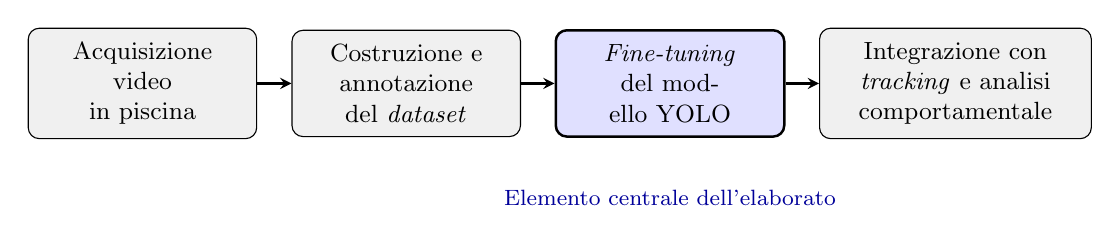
\begin{tikzpicture}[
        process/.style={draw, rounded corners, align=center, minimum height=1.35cm, text width=2.55cm, inner sep=5pt, font=\small},
        arrow/.style={->, >=stealth, thick}
        ]
        \node[process, fill=gray!12] (video) at (0,0) {Acquisizione video\\in piscina};
        \node[process, fill=gray!12] (dataset) at (3.35,0) {Costruzione e\\annotazione del \emph{dataset}};
        \node[process, fill=blue!12, line width=0.9pt] (yolo) at (6.7,0) {\emph{Fine-tuning}\\del modello YOLO};
        \node[process, fill=gray!12, text width=3.1cm] (pipeline) at (10.325,0) {Integrazione con\\\emph{tracking} e analisi comportamentale};
        
        \draw[arrow] (video) -- (dataset);
        \draw[arrow] (dataset) -- (yolo);
        \draw[arrow] (yolo) -- (pipeline);
        
        \node[font=\footnotesize, text=blue!60!black, align=center] at (6.7,-1.45) {Elemento centrale dell'elaborato};
    \end{tikzpicture}
    \caption{Schema ad alto livello del perimetro dell'elaborato}
    \label{fig:perimetro-elaborato}
\end{figure}

Il progetto assume infine come riferimento la norma UNI EN ISO 20380:2018, che definisce requisiti e procedure di prova per i sistemi di visione computerizzata destinati alla rilevazione di incidenti da annegamento nelle piscine pubbliche \cite{UNI20380}. La norma orienta le scelte progettuali, ma non viene perseguita né dichiarata una certificazione formale di conformità.

L'obiettivo è pertanto valutare l'idoneità di un modulo di \emph{object detection} all'interno di un sistema più ampio, considerando l'accuratezza, la capacità di generalizzazione, la velocità di inferenza e la compatibilità con le elaborazioni successive.

\section{Struttura dell'elaborato}

Il presente elaborato è articolato in sei capitoli. Dopo questa introduzione, il Capitolo~2 espone i fondamenti teorici necessari, descrivendo l'architettura generale di DEWS, il funzionamento di YOLO e le motivazioni che hanno condotto alla sostituzione del modulo di rilevazione originale. Il Capitolo~3 illustra il processo di realizzazione del \emph{dataset}, dalla fase di acquisizione fino all'annotazione e alla suddivisione nei diversi sottoinsiemi. Il Capitolo~4 descrive il processo di \emph{fine-tuning} e analizza sperimentalmente le prestazioni dei modelli considerati. Il Capitolo~5 affronta l'integrazione del modello selezionato all'interno della \emph{pipeline} esistente e ne valuta l'impatto. Infine, il Capitolo~6 riassume i risultati ottenuti, i limiti riscontrati e i possibili sviluppi futuri.
